\documentclass[10pt,a4paper]{article}

\usepackage{fullpage}
\usepackage{wrapfig}
\usepackage{lipsum}
\usepackage{hyperref}
\usepackage{cleveref}
\usepackage{tikz}
\usepackage{float}

\DeclareGraphicsExtensions{.pdf,.png,.jpg}

\begin{document}
\title{WebApp Group 34 Milestone Report}
\author{
  Han, Qiao\\
  \and
  Chabierski, Piotr\\
  \and
  Smith, Bradley\\
  \and
  Cingillioglu, Nuri\\
}

\maketitle

\section{Group Structure and Work Division}

\noindent
We divided our group responsibilities based on our individual strengths. Han has done extensive development work on both server and client side applications in past internships and part time jobs and is hence the most suitable candidate for the role of group leader. The group leader is responsible for guiding the choices of technology together with ensuring a schedule for the timely completion of the project. In addition, he is also responsible for managing the team during evaluations of the project requirements and the suitability of different technology stacks in fulfilling our design goals.
\\
\\
\noindent
More specifically, our team members are initially in charge of working on following areas.

\begin{enumerate}
  \item Client-side presentation - Nuri
  \item Client-side interaction - Nuri / Han
  \item Server-side processing - Bradley / Piotr / Han
  \item Database set-up - Bradley / Piotr
\end{enumerate}
\noindent
As we progress, we believe we will work on different parts of the project from this initial assignment so that everyone can get a holistic understanding of the full stack web application design.


\section{Choice of Implementation Languages}
Although the frontend has to be written in HTML, CSS, and Javascript, there exists a wide variety of web development frameworks that we have considered, ranging from full blown MVC models such as AngularJS, MeteorJS, Backbone.js, to minimalistic libraries such as jQuery, Modernizr, HTML5 Boilerplate. As the team is relatively new to web development, we decided to use frameworks that more closely represent the fundamental DOM layout to enhance our understanding. This means that HTML5 Boilerplate is a good choice because it modernises the standard HTML technologies without adding extra layers of abstractions. In addition, we have chosen to use the Bootstrap framework to enhance the visual presentation of our web app. Lastly, we have decided to separate our data models from the views by making AJAX calls to our backend using a RESTful API that retrieves JSON objects for updating the views. Using JSON as the data format is not only easy to parse and understand but also allows for rich data structures like nested objects and arrays.
\\
\\
\noindent
We have picked Java as our backend implementation language, after considering the strengths and weaknesses of Python, node.js, and PHP in detail.
Although it may increase the amount of time that writing our App will take, we believe this to be a good trade-off. Java code is much more habitable and allows for easier extension. We think it will keep our options open going forward as it is very portable and platform independent. Java also provides several frameworks we can use to unit test our code such as JUnit and Mockito along with many useful libraries to provide much of the functionality that we will need. We set up our web container using Apache Tomcat as it allows us to work in pure Java.
\\
\\
\noindent
Lastly for the database we chose to use PostgreSQL due to convenience as CSG had already given us an already configured database to use.  

\section{Description of our App}
Our project is a multi-user calendar App which allows people to, create/subscribe to calendars, create/join events and obtain feedback on who has signed up to your events. The App is targeted at volunteers for college events but can be easily extended for more general purposes.
\\
\\
\noindent
It has three main entity types and several relations between them, these are the users, the calendars and the events, see ~\cref{sec:er} for more details. The idea came from a specific problem that we found occurring very often, people using emails to organise events and work out specifically who can attend or to get a general idea of how many people to expect. This can lead to very inefficient communication and cause a verity of problems to occur. Such as events occurring so often that the people who are attending (volunteering) start to pay less attention to them, or if an event if so popular that it ends up being over subscribed and the organisers have to send a huge number of emails back to the people who didn't make it in time.
\\
\\
\noindent
We are designing and making our App while having these problems in mind and aim to come up with a system which could eliminate or ease some of them.

\section{User Interactions} 
The basic idea is that there will be two types of users (per calendar), the administrators and the users (subscribers). They will both interact with the calendars in different ways and have various typical uses. Note that any user can create a calendar or join others so these roles are not absolute.
\\
\\
\noindent
For the subscribers of calendars that need to be able to see events in a clear manner and easily be able to gauge their interest about the event. They also need the ability to sign up for the event if they wish to attend (depending on the event this might be a strict attendance or a flexible one). In addition to this they should be able to change between the calendars they are subscribed to and create a view with the calendars that interest them at any time. Finally they should be able to create calendars and gain administrator privilege on them. 
\\
\\
\noindent
The administrations of a calendar need extra abilities in addition to those of a subscriber. They will be able to create, modify details of and delete any event on their calendars along with the ability to see the number of people who have signed up and their identities. In addition they can delete whole calendars and invite people to subscribe via an invite code which they can give out to anyone who may be interested. We are also looking into other ways that users may be invited to calendars.  
\\
\\
\noindent
Lastly everyone will also be able to interact by registering and logging in to our App, see ~\cref{sec:fd} for user flow diagrams.

\appendix
\label{appendix}

\section{System Entities and Relations} 
\label{sec:er}
\begin{figure}[H]
\centerline{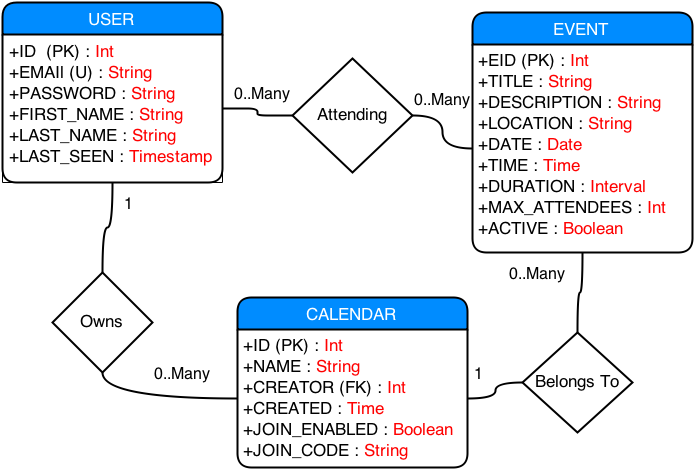
\includegraphics[scale=0.58,trim=0 0 100 0]{er}}
\caption{Entity Relation diagram with possible database layout}
\end{figure}
PK, FK and U stand for Primary Key, Foreign Key and Unique respectively. PK implies U.
\\
\\
\noindent
There is a relationship missing from this diagram, this is the subscriber relationship. Each of the relationships will be represented in the database as a table with ID to ID mappings with the 2 participants. The cardinality constraints can also be very easily added into the database to ensure that the data remains consistent. For example the \textbf{belongs to} relationship will be realised with a table with one column being the CID (Calendar Id) and the other being the EID (Event Id). The (CID,EID) pair will be the primary key.
\newpage
\section{User Interaction Diagrams}
\label{sec:fd}
\begin{figure}[H]
\centering
\begin{minipage}{.4\textwidth}
  \centering
  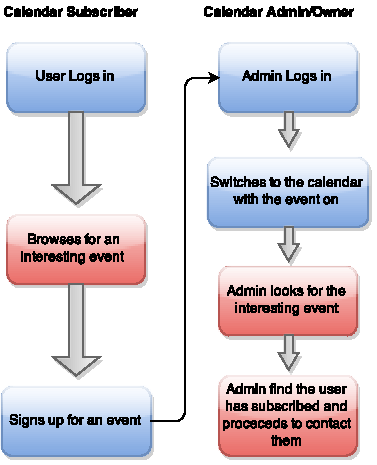
\includegraphics[width=1\linewidth]{user_event}
  \caption{Use flow of a user signing up}
\end{minipage}%
\begin{minipage}{.7\textwidth}
  \centering
  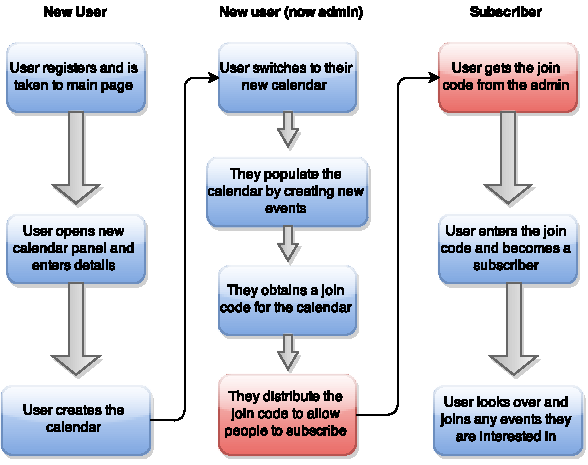
\includegraphics[width=0.9\linewidth]{calendar_user}
  \caption{Use flow of a new user creating a calendar}
\end{minipage}
\end{figure}
\noindent These diagrams show two typical use situations it which the user would interact with our WebApp. The blue boxes are explicit interactions with our App, where as the red boxes are events which require no explicit (but most like some) interaction.

\end{document}
